% !TEX root = ../lectures_olympics.tex

\chapter{万有引力理论}

\section{万有引力的发现}
牛顿建立动力学的根本原因就是为了解释长期的天文观测结果。
经过近百年的数据积累,摆在牛顿面前行星运动的规律由天文学家开普勒给出,被称为开普勒三定律:
\begin{enumerate}
\item 行星围绕太阳转动的轨道为椭圆,太阳在椭圆的一个焦点上。
\item 行星与太阳连线在相同时间里扫过相同的面积。
\item 行星公转周期的平方与轨道椭圆长轴的立方之比对于所有行星都相同。
\end{enumerate}
在学习牛顿定律的时候我们知道,当知道了物体的运动之后就可以根据牛顿第二定律得到物体所受力的大小。
对于行星或者其它天体也是一样的,从开普勒定律出发可以得到太阳与行星之间的作用力。

三个定律当中最直接的当属开普勒第二定律,由它可知行星运动过程中天阳和行星之间的作用力必然沿着它们之间连线的方向,如果认为太阳近似不动,那么行星的公转过程中受到的是时刻指向太阳的吸引力作用。

\begin{figure}
\begin{center}
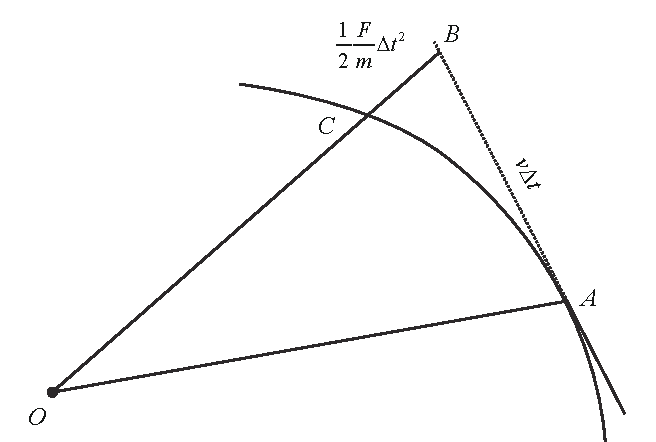
\includegraphics[width=0.5\textwidth]{images/gravity-1.pdf}
\caption{根据轨迹和面积速度求作用力}
\label{fig: 根据轨迹和面积速度求作用力}
\end{center}
\end{figure}

开普勒第一定律能够使我们知道太阳作用于行星时刻指向太阳的力反于于它们之间距离的平方。
这一点不借助一些数学工具很难直接看出来,而且在牛顿那个时代根本不存在这样的数学工具,这也就是牛顿发明微积分的主要动机。
在此我们简单地介绍一下牛顿所使用的方法,而真正的计算放在我们完整地学完微积分之后再进行。
我们知道,不受力的物体将会匀速直线运动,而受到外力作用时,当外力的方向与速度方向不一致时运动轨迹将会发生偏转。
最终物体运行的轨迹由惯性和外力共同决定,假设在某一给定时刻$t$,物体处于图\ref{fig: 根据轨迹和面积速度求作用力}中的$A$点,在它上面有时刻指向$O$点的力的作用,而在此后的$\dt$时刻它所处的位置由
\begin{equation}
\vec{r}(t+\dt)=\vec{r}(r)+\vec{v}\dt+\frac{1}{2}\frac{\vec{F}}{m}\dt^2
\end{equation}
给出。
对于给定轨道的运动,因为我们在前面已知作用力为有心力,所以矢径在单位时间里扫过的面积都相同,可以通过观测找到这个面积速度。
这样当质点处于某一给定点$A$时,在无外力作用时它将由于自己的速度运动到$B$点,两点之间的距离为$v\dt$。
由于向心力的作用,它实际上到达了图中的$C$点,且$BC$之间的距离为$\frac{1}{2}a\dt^2$,当轨迹和$O$点的位置都已知时,$BC$的长度可完全确定,这样比较两式就可知物体加速度的大小。
当轨迹为椭圆,$O$点位于椭圆的焦点时,可以证明此时行星所受力的大小反比于它到太阳距离的平方:
\begin{equation}\label{eqn: 反比于距离平方的作用力}
F = \frac{C}{r^2}
\end{equation}
对于单个行星无法确定比例常数$C$的大小。

为了确定这个比例系数,就必须借助开普勒第三定律。
对于每个行星可以根据它自身的轨道和周期得到它和太阳之间吸引力所对应的比例系数。
由于椭圆的几何性质可知每个行星所对应的$C$的值必须正比于它自身的质量。
椭圆比较复杂,实际上行星的轨道非常接近于圆形,可以用圆形做近似。
这时太阳将位于圆心处,轨道的半长轴就是圆的半径,对于半径为$R$,质量为$m$的行星,如果它和太阳之间引力\ref{eqn: 反比于距离平方的作用力}系数为$C$时,它做圆周运动需要满足
\begin{equation}
\frac{C}{r^2}=m\frac{v^2}{r}
\end{equation}
这样可以得到它圆周运动的周期
\begin{equation}
T=\frac{2\pi R}{v}=2\pi\sqrt{\frac{mR^3}{C}},
\end{equation}
这样它的周期和半长轴的比值就是
\begin{equation}
\frac{T^2}{R^3} = \frac{4\pi^2\frac{mR^3}{C}}{R^3}=\frac{4\pi^2m}{C}
\end{equation}
根据开普勒第三定律,所有行星的这个比值都为常数,所以对于每个行星来讲,它所受到的引力\ref{eqn: 反比于距离平方的作用力}必须正比于它自己的质量:
\begin{equation}
F = \frac{C}{r^2}=\frac{C'm}{r^2}
\end{equation}

这是开普勒三定律所能够告诉我们的全部。
再根据牛顿第三定律,这样的引力是存在于太阳和行星之间的,大小相等方向相反。
这样比例系数仅仅依赖于行星的质量从逻辑上就有些站不住脚。
另外通过对行星和它们的卫星的轨道和周期的观测发现行星和卫星之间的吸引力也满足类似的特征,比例系数则正比于卫星的质量。
这时将上面的结论稍做推广,并且一般化,就得到了牛顿著名的万有引力定律,指出自然界任何两个物体之间都存在有沿着彼此连线方向吸引力的作用,大小正比于两者质量的乘积,反比于它们之间距离的平方,比例系数对于所有的物体均相同:
\begin{equation}\label{eqn: 万有引力定律}
F = \frac{Gm_1m_2}{r^2}
\end{equation}
其中$m_{1,2}$分别为两个物体的质量,$r$为两者的距离,$G$为普适的比例常数,在国际单位制中它的大小约为
\begin{equation}
G\simeq 6.6\pow{-11}\unit{m^3kg^{-1}s^{-2}}
\end{equation}

\section{不能看做质点物体之间的引力}
原则上讲只有两个能够看做质点的物体之间的引力满足\ref{eqn: 万有引力定律},对于那些不能够看做质点的物体之间的引力的确定道理上其实也并不复杂,就是将它们分成很多的小部分,每一部分都可以看做是一个质点,这样两个物体之间的引力不是别的,正是小部分之间引力的矢量和。
对于那些密度均匀、形状规则的物体之间的引力我们是有机会算出它们之间的引力。

\begin{example}
试证明一个密度均匀的球壳对其内部质点的引力为零,对其外部质点的引力和一个质量相同、位于球心的质点的引力完全相同。
\tagged{student}{\vspace*{4cm}}
\begin{taggedblock}{teacher}
\newline
解析:略
\end{taggedblock}
\end{example}

\begin{example}
试证明一个距离球心相同距离处密度相同的球体(密度球对称分布)对其外部质点的引力等于一个质量相同,位于球心的质点所产生的引力相等。
\tagged{student}{\vspace*{4cm}}
\begin{taggedblock}{teacher}
\newline
解析:略
\end{taggedblock}
\end{example}

\begin{example}
在一个半径为$R$,密度为$\rho$的均匀实心球内部掏一个半径为$0.5R$的球形空穴,并与大球相切。
一个质点$m$位于空穴内部,(1)试求$m$在空穴中心受到的万有引力,(2)证明$m$在空穴任意位置受的引力处处一样。
\tagged{student}{\vspace*{4cm}}
\begin{taggedblock}{teacher}
\newline
解析:假设一个质量为负的球和质量为正的球叠加
\end{taggedblock}
\end{example}



\section{万有引力定律的一些结论}
地球表面的重力实际上就是地球和地表物体之间万有引力的一种表现形式,在地球附近质量为$m$的物体受到引力的大小为
\begin{equation}
F = \frac{GM_Em}{R_E^2}
\end{equation}
其中$M_E$、$R_E$分别代表地球的质量和半径。
当物体的高度变化与地球半径相比可以忽略不计时,它受到的引力可以近似地用
\begin{equation}
F = mg,\qquad g = \frac{GM_E}{R_E^2}
\end{equation}
来代替,其中$g$就是熟知的地球表面的重力加速度。


\begin{example}
试求一个地球表面附近的物体为了能够围绕地球做圆周运动所需要的具有的速度。这个速度被称为地球的第一宇宙速度。
\tagged{student}{\vspace*{4cm}}
\begin{taggedblock}{teacher}
\newline
解析:$\sqrt{gR}$
\end{taggedblock}
\end{example}


\begin{example}
随着地表物体高度的升高,质量为$m$的物体和地球之间引力的大小与$mg$相差越来越大。
如果要求它们之间的差别不超过 1\%,那么它至多离地表多高?
忽略自球的自转、形状等因素。
\tagged{student}{\vspace*{4cm}}
\begin{taggedblock}{teacher}
\newline
解析:略
\end{taggedblock}
\end{example}

\begin{example}
已知火星的质量约是地球的$\frac{1}{10}$,半径约为地球的$\frac{1}{2}$,公转轨道约为地球的1.5倍。
根据以上数据试估计火星的相关参数和地球的比值:表面积、体积、密度、表面重力加速度、第一宇宙速度和公转周期。
假设火星和地球均为密度均匀的球形,公转轨道为正圆。
\tagged{student}{\vspace*{4cm}}
\begin{taggedblock}{teacher}
\newline
解析:略
\end{taggedblock}
\end{example}

引力是存在于所有物体之间的,在引力作用下所有物体都会获得加速度。
太阳系中太阳处于正中静止不动仅仅是一个近似,这是因为太阳的质量远远大于所有行星的质量,太阳系中最重的行星木星的质量也大约只有太阳质量的千分之一。
如果需要更准确地描写天体的运动就必须考虑所有物体之间的引力以及引力引起的加速度。

\begin{example}
我们知道月球在地球的引力作用下围绕地球转动。
其实和地球质量相比月球的质量不能够忽略不计,忽略其它天体的作用,假设轨道为圆形,求地球和月球互相围绕对方转动的中心距离地球中心的距离。
已知地球的质量$M_E\simeq 5.97\pow{24}\unit{kg}$,月球质量$M_M\simeq 7.34\pow{22}\unit{kg}$,地月距离$d\simeq 3.84\pow{5}\unit{km}$,地球半径$R_E\simeq 6370\unit{km}$。
试给出当假设地球静止不动时所得到的月球公转周期的误差。
\tagged{student}{\vspace*{4cm}}
\begin{taggedblock}{teacher}
\newline
解析:月亮不是绕着地球转,而是绕着地月系统的质心转,但是地球质量远大于月球。系统质心与地球的距离为$d'=\frac{M_M}{M_M+M_E}d$。由运动学有:$F=\frac{GM_EM_M}{d^2}=M_M\frac{2\pi}{T}^2d'$
\end{taggedblock}
\end{example}


\begin{example}
设某次天文观测的结果表明,太空中有一颗恒星独自在做半径为$r$,周期为$T$的圆周运动,通过它的其它天文现象推测它的质量为$m$。
这明显不符合运动定律,所以我们猜测在它旁边有一个黑洞的存在。
黑洞是这样一种天体,它的质量极大,其它天体能够感受到它的引力,但它本身并不发光不能够直接观测。
试根据观测数据确定该黑洞的质量。
\tagged{student}{\vspace*{4cm}}
\begin{taggedblock}{teacher}
\newline
解析:设黑洞的质量为M,$\frac{GMm}{r^2}=m\frac{2\pi}{T}^2r$
\end{taggedblock}
\end{example}

\section{引力作用下的运动:功、势能和角动量}
当两个物体的距离发生变化时,引力会做功,很明显当两者距离变小时引力做正功,反之将做正功。
两个质量分别为$m_{1,2}$的物体由距离$r_1$变为$r_2$时引力做功的大小为
\begin{equation}
W = Gm_1m_2\left(-\frac{1}{r_1}+\frac{1}{r_2}\right).
\end{equation}
很明显可以看出引力做功的大小仅仅依赖于两者之间的距离,可知引力是一个保守力,可以定义两者之间的引力势能为
\begin{equation}
E_p(r)=-\frac{Gm_1m_2}{r}
\end{equation}
这里我们将势能的零点选在了无限远处。

\begin{example}
一个距离太阳$r$,质量为$m$,速度为$v_0$的天体,如果它的能量足够大,能够脱离太阳引力而飞向外太空,求它在距离太阳非常远的距离处速度的大小。
\tagged{student}{\vspace*{4cm}}
\begin{taggedblock}{teacher}
\newline
解析:$\frac{1}{2}mv_0^2-\frac{GMm}{r}=\frac{1}{2}mv^2$
\end{taggedblock}
\end{example}

\begin{example}
地面上竖直放置一根质量为$m$长为$L$的均匀杆,其长度与地球半径相比不可忽略不计。
如果将它以给定的速度$v_0$匀速升起,试求作用在它上面的合外力的功率与它的底部离开地面的高度的关系。
\tagged{student}{\vspace*{4cm}}
\begin{taggedblock}{teacher}
\newline
解析:$F=\frac{GMm}{L}(\frac{1}{R+h}-\frac{1}{R+L+h})$
功率 $W=F*v_0$
\end{taggedblock}
\end{example}

如果两个物体之间仅仅存在有引力作用,那么总的机械能守恒。
简单起见我们假设其中一个物体的质量远远大于另一个物体的质量,这样两者的引力对大质量物体的影响可以忽略不计,可近似将其看成是静止不动。
设大质量物体的质量为$M$,小质量物体的质量为$m$,这样的近似下,整个系统的机械能为第二个物体的动能和两者这间的引力势能之和:
\begin{equation}
E = \frac{1}{2}mv^2-\frac{GMm}{r}
\end{equation}
这样只要知道了整个系统的总能量就可知质量为$m$的物体在任意距离处的速度大小。

更进一步,当假设大质量为物体在空间中静止不动时小物体受到的引力可以看做是一个有心力,它相对于大质量质点所处位置角动量守恒。
在任意位置将$m$的速度分解为径向速度$v_r$和$v_\perp$时,它的角动量可以表达为
\begin{equation}
L = mv_\perp r
\end{equation}
其中$r$为$m$与$M$的距离。

不求解运动方程,仅仅段依靠能量守恒和角动量守恒就可以得到很多重要的结论。
在角动量的学习中我们已经见过了一些在反比于距离的势能下运动的性质,其实只需要将那里的比例系数用引力定律做替换即可。

\begin{example}
地球表面的物体的速度至少要达到多少才能够完全脱离地球引力而飞向无限远处。
这个速度被称做第二宇宙速度。
根据前面给出火星的数据求火星的第二宇宙速度。
\tagged{student}{\vspace*{4cm}}
\begin{taggedblock}{teacher}
\newline
解析:$\sqrt{2gR}$
\end{taggedblock}
\end{example}


\begin{example}
两个质量分别为$M$和$m$的天体在彼此之间引力下运动且$M\gg m$,设在某一时刻$m$与$M$的距离为$r_0$,速度$v_0$垂直于两者连线的方向。
如果此后$m$的速度与$M$可以再次垂直,求出它们之间的距离以及$m$的总机械能。
给出此后$m$的速度与$M$不会出现再次垂直的情况$m$的总机械能需要满足的条件。

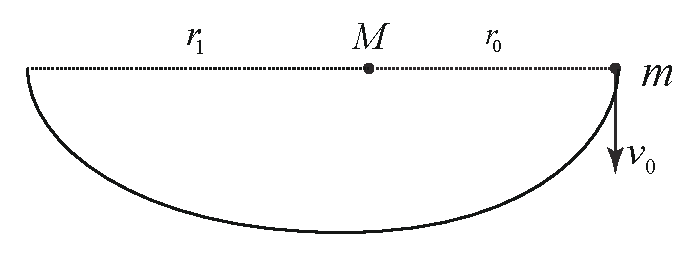
\includegraphics[width=0.3\textwidth]{images/gravity-ex2.pdf}
\tagged{student}{\vspace*{4cm}}
\begin{taggedblock}{teacher}
\newline
解析:总机械能小于0,能再次垂直。总机械能不小于0,会飞到无穷远处再也不回来。
\end{taggedblock}
\end{example}



\section{一些数学:椭圆和圆椎曲线}
开普勒第一定律告诉我们在平方反比的引力作用下的物体沿椭圆轨道运动。
为了进一步研究引力运动下的运动,我们必须学习一些椭圆的性质。
一个椭圆如下图所示,图中$OA=a$称为椭圆的半长轴,$OB=b$为椭圆的半短轴,另外在椭圆上还有两个特殊点$C$和$C'$,它们称之为椭圆的焦点。
一个椭圆可由如下的方式定义
\begin{description}
\item[圆投影]
一个椭圆可以看做一个圆在某一给定角度$\theta$在一个平面上投影所产生的图形。
其于这样的定义我们可知短轴
\begin{equation}
b=a\cos\theta,
\end{equation}
而且椭圆的面积也可以通过投影的定义轻易地得到:
\begin{equation}
S_e=\pi ab.
\end{equation}
\item[圆椎截面]
椭圆、抛物线和双曲线统称为圆椎曲线,考虑一个对顶的无限长圆椎,任何一种圆椎曲线都可以看做是一个平面与对顶圆椎相交的轨迹。
\item[焦点性质]
一个椭圆还可以定义为到平面上给定两个点之间距离之和等于给定常数所有的点所构成的几何图形。
这两个点被称为椭圆的焦点,而这个给定的距离很容易证明,它等于椭圆的长轴$2a$。
两个焦点距离的一半称做焦距$c$,它和长轴、短轴之间满足
\begin{equation}
c^2=a^2-b^2
\end{equation}
还可以定义椭圆的偏心率$e$为焦距和半长轴$a$的比值,从定义可以看出偏心率等于零的椭圆实际上就是一个圆,而随着偏心率的增大椭圆则看上去越来越扁。
\item[直角坐标系]
在一个直角坐标系中,如果把椭圆的中心放在原点,横轴放于$x$上时椭圆上的所有点由方程
\begin{equation}
\frac{x^2}{a^2}+\frac{y^2}{b^2}=1
\end{equation}
所给出,从中也可以看出当长轴与短轴相等时实际上就是一个圆。
\item[极坐标系]
如果把椭圆的一个焦点放在平面极坐标系的原点,而长轴放在极坐标系的参考线上时,椭圆可以表达成
\begin{equation}
r = \frac{\rho}{1+e\cos\theta}
\end{equation}
其中$\rho$是某一参考长度,$\theta$则是对应点的角度,而$e$不是别的,正是椭圆的偏心率。
其实不仅仅是椭圆,其它的圆椎曲线也可以用同样的方程来给出,只不过偏心率的取值范围有所不同。
\end{description}

\begin{example}
引力作用下的椭圆轨道由两个参数所决定,对于我们来说最方便的选择自然是椭圆的半长轴$a$和偏心率$e$。
它们由物体的性质所决定,对于天体或人造飞行器来说最基本的两个物理量就是它们的能量$E$和角动量$L$,因为它们两个是运动的守恒量。
试证明一个质量为$m$的物体在一个质量$M$物体的引力作用下轨道参数和运动学变量之间满足
\begin{equation}\nonumber
a=-\frac{GMm}{2E},\qquad e=\sqrt{1+\frac{2L^2E}{G^2M^2m^3}}
\end{equation}
并尽可能详细地讨论轨道和$E$和$L$的关系。
\tagged{student}{\vspace*{4cm}}
\begin{taggedblock}{teacher}
\newline
解析:略
\end{taggedblock}
\end{example}



%%%%%%%%%%%%%%%%%
\begin{example}

从赤道上的$C$点发射洲际导弹,使之精确地击中北极点$N$,要求发射所用的能量最少。
假定地球是一质量均匀分布的半径为R的球体,$R=6400\unit{km}$。
已知质量为$m$的物体在地球引力作用下作椭圆运动时,其能量$E$与椭圆半长轴$a$的关系为
\[
E = -\frac{GMm}{2a}
\]
式中$M$为地球质量,$G$为引力常量。

(1)假定地球没有自转,求最小发射速度的大小和方向(用速度方向与从地心$O$到发射点$C$的连线之间的夹角表示)。

(2)若考虑地球的自转,则最小发射速度的大小为多少?


\tagged{student}{\vspace*{4cm}}
\begin{taggedblock}{teacher}
\noindent
解析:(1)7.2km/s    (2)7.2km/s
\end{taggedblock}
\end{example}
%%%%%%%%%%%%%%%%%%%%%%


\begin{example}
当航天器的能量$E>0$时,其运动的轨迹并不是一个椭圆而是一条双曲线,数学上一条双曲线由$e>1$的圆椎曲线所给出。
当一个质量为$m$的飞行器由无限远以速度$v_0$向着一个质量为$M$的天体飞行,天体的中心与飞行器速度方向垂线的长度为$b$,试求在天体引力作用下飞行器再次飞行到无限远处的速度大小和方向的变化量。
为了使该变化量尽可能得大,飞行器的初始条件$v_0$,$b$应如何变化?
\tagged{student}{\vspace*{4cm}}
\begin{taggedblock}{teacher}
\newline
解析:双曲线知识是解题的必要条件。
根据动量守恒与能量守恒,得到速度达到最大时,航天器与飞船的距离为r,解出$\frac{1}{r}=\frac{GM}{v_0^2b^2}+\sqrt{(\frac{GM}{v_0^2b^2})+\frac{1}{b^2}}$
\\双曲线a,b,c。b=题目中的b。$c-a=r,c^2=a^2+b^2$  得到:$a=\frac{b^2-r^2}{2r}$ 。
转过的角度为$2\arctan\frac{b}{a}$ ,速度大小不变
\end{taggedblock}
\end{example}




%%%%%%%%%%%%%%%%%
\begin{example}

有一个办法可以不借助微积分来证明万有引力作用下行星公转的轨道为椭圆,为了发现这个事实请证明以下几个结论:

(1)如图所示,假设行星在其轨道上某一时刻与太阳之间的距离为$r$,其速度为$v$,$v$与$r$之间的夹角为$\theta$,如果行星的总能量为$E$,轨道角动量为$L$时,有如下的数量关系:
\[\sin^2\theta = \frac{\frac{L^2}{2m}}{Er^2 +GMmr}\]

(2)在一个半长轴为$a$,偏心率为$e$的椭圆上任意一点处做切线,切线与该点到椭圆的一个焦点连线方向的夹角为$\theta$,连线长度为$r$,证明如下的关系:
\[
\sin^2\theta = \frac{(1-e^2)a^2}{-r^2+2ar}
\]

(3)通过比较两式你能够得到轨道是椭圆的结论吗?如果可以,请给出椭圆参数$a$和$e$与行星的动力学参数$E$和$L$的关系。
\begin{center}
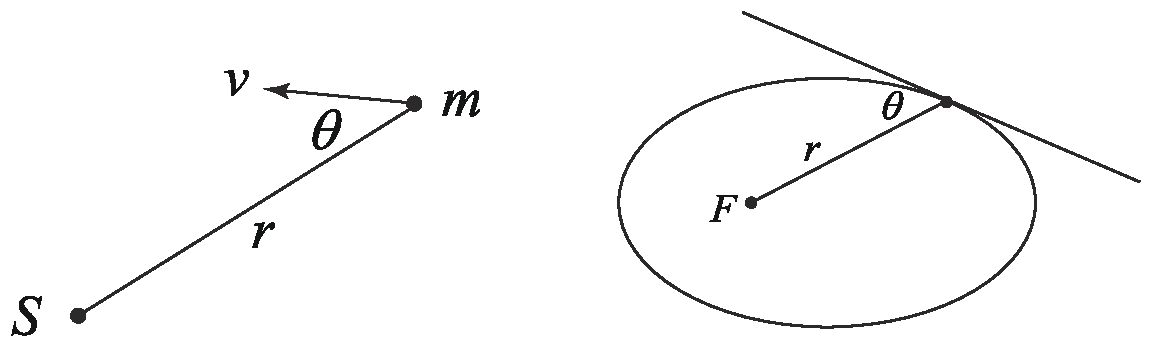
\includegraphics[width = 0.6\textwidth]{images/gravity-2.pdf}
\end{center}
\tagged{student}{\vspace*{4cm}}
\begin{taggedblock}{teacher}
\noindent
解析:略
\end{taggedblock}
\end{example}
%%%%%%%%%%%%%%%%%%%%%%

\section{航天器的轨道}
在引力作用下人造飞机器的运动是一个重要的问题,尤其是在空间时代我们能够使人造的飞机器飞向更远的天体,甚至已经快飞出了太阳系。
但是一般来说航天器轨道的计算十分复杂,而现在工程师已经有成熟的计算技术利用大型计算机精确地计算出人造卫星运动的每个细节,不过对于我们现在来说并不具备这样专门的技术,利用引力的基本性质部分地计算航天器轨道的部分特点还是一件很有意思的事情。
这时需要针对具体的问题进行分析,充分利用各种守恒定律以及准确的计算就可以得到结果。
这里我们看和几种经典的飞行相关的问题。

\begin{example}
为了使航天器完全脱离太阳引力而飞出太阳系之外所需的最小相对地球的发射速度为多少?
这个速度被称为第三宇宙速度。
\tagged{student}{\vspace*{4cm}}
\begin{taggedblock}{teacher}
\newline
解析:16.7km/s 倒着推。
\end{taggedblock}
\end{example}

\begin{example}
假设开始时刻有一颗人造卫星位于距地心$r$的轨道上做匀速圆周运动,为了改变该卫星的轨道,使其轨道的近地点与地球相切,我们需要对其进行加速。

(1)如果沿着卫星运行速度的方向喷气,那么所需要它的速度改变量为多大?这时推进器对航天器做功为多少?

(2)如果沿着卫星与地球连线方向喷气,那么所需要的速度改变量为多少?
\tagged{student}{\vspace*{4cm}}
\begin{taggedblock}{teacher}
\newline
解析:(1)$\Delta v=\sqrt{\frac{2GM}{r}}-\sqrt{\frac{2GMR}{r(r+R)}}$
\\(2)$\Delta v=\sqrt{\frac{2GM}{r+R}}$
\end{taggedblock}
\end{example}


\begin{example}
已知地球和火星都在同一平面上绕太阳做圆周运动,火星轨道半径$R_m$为地球轨道半径$R_0$的1.5倍。
若要从地球表面向火星发射探测器,简单而又比较节省能量的发射过程可分为两步:
\\1.在地球表面用火箭对探测器进行加速,使之获得足够的动能,从而成为一个沿地球轨道运行的人造行星(此时,地球对探测器的引力很小,可以忽略不计)。
\\2.在适当时刻点燃与探测器连在一起的火箭发动机,在短时间内对探测器沿原运动方向加速,使其速度数值增加到适当值,从而使得探测器沿着一个与地球轨道及火星轨道分别在长轴两端相切的半个椭圆轨道上运动,从而使探测器正好射到火星上,如图所示。已知$R=6.4*10^6m$ ,$g=10m/s^2$求:
\\(1)为使探测器成为绕地球运行的人造卫星,探测器在地面附近至少要获得多大的速度(不考虑地球自转)。
\\(2)求火星探测器的飞行时间为多少天。
\\(3)当探测器脱离地球并沿地球公转轨道稳定运行后,在某年3月1日零时,经观测计算知火星与探测器与太阳所张角度为60$^\circ$。问应在何年何月何日点燃探测器上的火箭发动机方能使探测器恰好落在火星表面(时间计算仅需精确到日)。
\begin{flushright}
		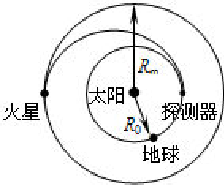
\includegraphics[width = 0.2\textwidth]{images/gravity-3.pdf} 
	\end{flushright}
\tagged{student}{\vspace*{4cm}}
\begin{taggedblock}{teacher}
\noindent
解析:(1)8.0km/s
(2)251天
(3)4月11日
\end{taggedblock}
\end{example}


\begin{example}
其实在前面算出的第三宇宙速度并不是能够使航天器飞出太阳系所需要的最小速度,只要轨道设计地足够好,其实还可能得到更小的发射速度。
这时我们可以借助其它天体的引力使航天器的飞行过程中再次被加速度,这种效应被称做引力弹弓。
这里我们希望借助木星的引力弹弓效应,那么相对地面最小的发射速度可以变成多少?
\tagged{student}{\vspace*{4cm}}
\begin{taggedblock}{teacher}
\newline
解析:略
\end{taggedblock}
\end{example}

\section{引力作用下的天体运动}
虽然引力定律并不复杂,但如果考虑在引力作用下的天体的运动有时也不是那么简单,需要在利用运动规律的基础上同时也注意各个物理量如何定义,如何变化,达到特定的状态时需要满足什么条件。
对于引力作用下的天体运动人们始终想找到精确的解,经过数百年的努力最终终于认识到哪怕是只有三个物体在彼此之间万有引力作用下的解析解也是不存在的,这就是著名的三体问题。
尽管如此,我们还是可以忽略质量相对较小的天体引力作用,这时就可以得到近似的运动。
我们来看几个简单的情况。





\section{地-月系统}
早在上古时代人们就已经对天空最大的月球充满了无限的向往,并对月球进行了精确地观测。
如果仅把考虑地球和月球看做一个孤立系统的话,月球的运动并不复杂,可以认为月球的运动与开普勒定律给出的结果一致。
但是实际上由太阳的引力对月球绕地球的公转的偏差并不能够完全忽略,它所引起的效果很早人们就已经注意到了。
从牛顿建立力学定律以后人们对在太阳引力干扰下月球的运动的计算做了大量的工作,但是直到二百多年之后才得到了第一本能够用于航海的月球星表,可见其复杂程度。
我们现在不可能进行类似的计算,但依然可在我们知识范围内推出很多地球和月球在它们之间引力作用下造成的可观测现象。
比如说著名的潮汐现象
\begin{example}
假设地球是一个完全由水包裹着的星球,在月球引力作用下地球表面的水面并不是完全的正圆。
试求平衡状态下地球上的水面距离地心的距离最大值与最小值的差。
\tagged{student}{\vspace*{4cm}}
\begin{taggedblock}{teacher}
\newline
解析:$h=\frac{R^4}{d^3}\frac{m}{M}$ 
潮汐高度等于地球半径的四次方、除以月地距离的三次方、乘以月球与地球的质量比,约为0.4m。
\end{taggedblock}
\end{example}


\begin{example}
试定性地解释为什么月球总是一面向着地球。
\tagged{student}{\vspace*{4cm}}
\begin{taggedblock}{teacher}
\newline
解析:潮汐,摩擦,减速。
\end{taggedblock}
\end{example}













